\documentclass[a4paper, 14pt]{article}

\usepackage[utf8]{inputenc}
\usepackage{graphicx}
\usepackage{float}%"Плавающие" картинки
\usepackage{wrapfig}%Обтекание фигур (таблиц, картинок и прочего)
\usepackage{amsmath, amssymb, amsthm}
\usepackage[T1, T2A]{fontenc}
\usepackage[english, russian]{babel}
\usepackage[left=2cm,right=2cm, top=2cm, bottom=2cm]{geometry}
% Литература в biblatex
\usepackage[backend=biber,bibencoding=utf8,language=auto,autolang=other,sorting=ntvy,babel=other,
            maxbibnames=99,maxcitenames=2,style=gost-numeric,movenames=false]{biblatex}
\addbibresource{../doc/refs.bib}
% Межстрочный интервал = 1.5pt
\usepackage{setspace}
\onehalfspacing
% % Абзацный отступ = 1.25см
\usepackage{indentfirst}
\setlength\parindent{12.5mm}
% Путь до папки с изображениями
\graphicspath{ {./images/} }
% Активные ссылки на формулы и лит-ру
\usepackage[
  colorlinks=true,
  citecolor=blue,
  linkcolor=blue,
  linktoc=page,
]{hyperref}
% tilde symbol
\usepackage{textcomp}
\renewcommand{\texttilde}{\raisebox{0.5ex}{\texttildelow}}
% Reynolds number
\newcommand{\Ren}{\mathrm{Re}}
\renewcommand{\vec}[1]{\boldsymbol{\rm #1}}

\begin{document}

\begin{titlepage}
\begin{center}

\hfill \break

\large{Министерство науки и высшего образования Российской~Федерации}\\
\footnotesize{Федеральное государственное автономное образовательное учреждение высшего образования}\\ 
\small{\textbf{«КАЗАНСКИЙ (ПРИВОЛЖСКИЙ) ФЕДЕРАЛЬНЫЙ УНИВЕРСИТЕТ»}}\\

\hfill \break
\normalsize{Институт механики и математики им. Н. И. Лобачевского}\\

\hfill \break
\normalsize{Направление подготовки: 01.01.03 Механика и математическое моделирование}\\

\vspace{25mm}
\large{Курсовая работа}\\
\end{center}

\vspace{20mm}
\noindent
Студентка 3 курса \\
группы 05-001 \\
<<\underline{\hspace{0,75cm}}>> \underline{\hspace{2cm}}\the\year~г.

\hfill \break
Научный руководитель \\
<<\underline{\hspace{0,75cm}}>>\underline{\hspace{2cm}}\the\year~г.

\vspace{\fill}

\begin{center}
    Казань, \the\year
\end{center}
\thispagestyle{empty}

\end{titlepage}


\newpage
\tableofcontents
\newpage

\section{Введение}
\subsection{Актуальность работы}

Кровь -- соединительная ткань внутри организма, она состоит из форменных клеток (эритроцитов, лейкоцитов, тромбоцитов), а так же из
водного раствора белков и свёртывающих веществ -- плазмы. Кровь под воздействием периодических сокращений сердечной мышцы 
движется по замкнутой системе сосудов, циркулируя от сердца и обратно. С точки зрения гидродинамики кровоток представляет 
из себя пульсирующее с низкой частотой течение мелкодисперсной суспензии в 
замкнутой системе каналов кругового сечения с эластичными стенками, осложнённое локальными эффектами ламинарно-турбулентного перехода.

Сложность разветвления кровеносных сосудов и вариации их размеров создают значительные трудности при решении задачи о течении крови. 
Математическое моделирование помогает  
аппроксимации и пониманию сложностей кровотока. Эти модели позволяют описывать и строить физические процессы, происходящие 
в биологических областях, что может быть полезно при выявлении, прогрессировании и лечении  различных сердечно-сосудистых заболеваний , 
а так же в проектировании и оптимизации медицинских устройств.

Описывать кровь можно различными способами. Например, детально: кровь состоит из взвешенных в плазме 
(которую чаще рассматривают, как ньютоновскую жидкость) клеток крови, которые действуют друг на друга с некоторыми силами. 
Описание такого типа методов можно подробнее изучить в ~\cite{Fedosov:2010,Fedosov:2008,Mehboudi:2001}. 
В некоторых моделях ~\cite{bessonov:2014,hosseini:2009} пренебрегают относительно мелкими и редкими -- тромбоцитами
(2--4~мкм в количестве 150--300 миллионов на 1~см$^3$) и лейкоцитами(4--20~мкм в количестве 4.5 -- 11 миллионов на 1~см$^3$), 
а строят двумерные сетки, состоящие только лишь из эритроцитов (7 -- 8~мкм в количестве 3.8 до 5.6 миллиардов клеток на 1~см$^3$).
Но при таких подходах можно столкнуться с некоторыми проблемами: такую модель будет сложно сравнивать как
с другими моделями, так и с эксперементальными показателями, так же она очень плохо реагирует на любые изменения в исходных данных. 
Соответсвенно, возникает необходимость прибегнуть к дальнейшему осреднению.

Можно не описывать индивидуальные частицы взвешенные в плазме, а обобщить их до вязкой неньютоновской жидкости с определёнными 
характеристиками, тогда любые изменения можно будет отразить в параметрах жидкости. Такой подход называют трехмерным моделированием.
Существует множество трёхмерных моделей, например, основанные на зависимости вязкости от гематокрита ~\cite{walburn:1976},
модель Максвелла \cite{thurston:1972},  модель Кассона ~\cite{moller:2006}.
Однако эти модели всё-таки требуют значительных вычислительных ресурсов, а следовательно, и дальнейших упрощений. 

Для вывода граничных условий в трёхмерных моделях иногда используют одномерное моделирование, которое может быть 
и вполне самостоятельным подходом к моделированию течения крови.
В одномерных моделях пространственные характеристики осредняются по поперечному сечению, а трёхмерная дифференциальная
задача сводится к одномерной. Такой подход к моделированию требует меньших вычислительных ресурсов, но при этом почти не уступает в 
точности другим моделям. О сравнении одномерных и многомерных моделей можно прочитать в ~\cite{FORMAGGIA:2001}.

В постановке задачи одномерного моделирования есть несколько ключевых аспектов. Первое -- 
определение геометрии сосудов: их длина, поперечное сечение, разветвлённость. Точность определения этих данных существенно влияет 
на результат моделирования. Для повышения точности геометрических данных сравнивают данные из различных
источников, используют МРТ и ультразвуковые исследования, а так же калибруют уже готовую модели. В работе 
\cite{Shanmugavelayudam:2010} рассматривают влияние геометрических допущений на численное моделирование.

Так же необходимо задать физические характеристики крови, такие как её плотность (обычно её оценивают в 1052 -- 1060~кг/м\textsuperscript{3}),
вязкость (4.3 -- 4.9~мПа$\cdot$с), состав крови (количество эритроцитов, лейкоцитов и тромбоцитов, увеличение или уменьшение ктороых
влияет и на другие физические характеристики. Подробнее в~\cite{Bouchnita2020}).

Кровь, двигаясь по сосудам, испытывает сопротивление движению со стороны сосудов и из-за своей вязкости. Поэтому сердце вбрасывает 
кровь в сосуды под большим давлением. В аорте давление колеблется в диапазоне от 120~мм рт.ст. при систоле до 80~мм рт.ст. при диастоле. 
По мере движения крови давление в сосудистом русле падает. 

Скорость течения крови так же зависит от диаметра сосуда, удалённости сосуда от сердца, а также фазы сердечного цикла. 
Максимальных значений скорость достигает в аорте (до \texttilde$1$~м/с), а минимальных -- в капиллярах (около нуля).
Линейная скорость в полых венах в два раза меньше, чем в аорте и равна примерно $2.5\cdot10^{-1}$~м/с, 
поскольку в организме на одну артерию приходится две вены.

Необходимо так же определиться и с граничными условиями. В общем случае: на входе задаётся  систолическое давление, 
а на выходе диастолическое. О влиянии граничных условий в задаче одномерного моделирования можно прочитать в~\cite{Krivovichev:2022}.

Для построения модели нужно выбрать подходящий метод. Метод конечных элементов~\cite{TAYLOR1998} -- популярная численная схема. 
Он особенно хорошо подходит для моделирования сложных геометрий, таких как запутанная сеть артерий в человеческом теле. 
Однако он может быть вычислительно дорогим, особенно для больших и сильно разветвленных сетей. 

Метод быстрого преобразования Фурье~\cite{Sazonov:2019} -- 
это подход, использующий быстрое преобразование Фурье для решения одномерных уравнений кровотока. 
Этот метод конкурирует с традиционными пространственно-временными численными схемами как по устойчивости, так и по скорости. 
Он может точно и эффективно обрабатывать сложные геометрические формы и высокоамплитудные волны. 
Однако он требует дальнейшего развития для учета вязкоупругих эффектов и потери массы крови из-за мелких ветвей. 

Метод прерывистого Галеркина~\cite{yao:2017} -- это еще одна численная схема, она сочетает в себе преимущества методов конечной разности и конечных элементов, 
обеспечивая баланс между точностью и вычислительными затратами. Однако он может быть более сложным в реализации и может
потребовать дополнительных вычислительных ресурсов для сопоставления расчетной и физической областей.

Метод конечных объемов с локальным временным шагом высокого порядка~\cite{mueller:2015} предполагает решение управляющих уравнений 
с помощью метода конечных объемов высокого порядка и схемы локального шага по времени. 
Этот метод может быть особенно полезен для моделирования течения в сложных геометрических системах.

Метод конечных разностей предполагает дискретизацию области на сетку точек и последующую аппроксимацию производных в управляющих
уравнениях с помощью конечных разностей. Этот метод часто используется в сочетании со схемой интегрирования по времени для решения 
полученной системы обыкновенных дифференциальных уравнений.




\section{Подходы к моделированию кровотока}
\subsection{Детальное моделирование}
Моделировать кровь можно как жидкость со взвешенными в ней клетками крови, которые могут рассматриваться, как совокупность частиц и сил,
действующих между ними. Эритроциты гораздо крупнее остальных клеток крови и они составляют большую часть её объёма, соответственно они 
и будут определять механические свойства крови. Плазма крови -- раствор крупных молекул, но при масштабах движения и при скоростях
сдвига, обычно встречающихся в кровеносных сосудах, ее можно считать однородной ньютоновской жидкостью  и описывать уравнениями
Новье-Стокса. То есть нам нужно учитывать взаимодействие частиц с жидкостью и друг с другом. Такую задачу удобно решать методом 
диссипативной динамики частиц.

Диссипативная динамика частиц -- это метод, в котором каждая частица описывает небольшой объем моделируемой среды, 
а не отдельную молекулу. Их взаимодействие определяется консервативными $F^C_{ij}$ (не зависящими от траектории), диссипативными 
$F^D_{ij}$ (силы, при действии которых полная механическая энергия  системы убывает, переходя в другие, не механические формы энергии) 
и случайными силами $F^R_{ij}$, действующими между двумя частицами:
\begin{align*}
  &\vec{F^C_{ij}}=F^C_{ij}(r_{ij})\vec{\hat{r}{_{ij}}},\\[10pt]
  &\vec{F^D_{ij}}=-\gamma \omega^D(r_{ij}) (\vec{v_{ij}} \cdot \vec{\hat{r}{_{ij}}})\vec{\hat{r}{_{ij}}},\\[10pt]
  &\vec{F^R_{ij}}=\sigma \omega^R(r_{ij}) \dfrac{\varepsilon_{ij}}{\sqrt{\bigtriangleup t}} \vec{\hat{r}{_{ij}}},
\end{align*}
где $\vec{r_{i}}$— радиус-вектор i-ой частицы, $\vec{r_{ij}}=\vec{r_{j}} - \vec{r_{j}}$,
$r_{ij}=|\vec{r_{ij}}|$,
$\vec{\hat{r}{_{ij}}}=\vec{r_{ij}}/{r_{ij}}$,
$\vec{v_{ij}}=\vec{v_{j} - \vec{v_{j}}}$ -- разница между скоростями двух частиц, $\bigtriangleup t$ -- шаг по времени, 
$\gamma, \sigma$ -- это  коэффициенты, определяющие силу диссипативной и случайной силы соответственно, а $\omega^R,\omega^D$ -- весовые функции,
${\varepsilon_{ij}={\varepsilon_{ji}}}$ -- нормально распределенная случайная величина с нулевым средним и единичной дисперсией.

Мембрана эритроцита практически несжимаема и устойчива к изменению площади поверхности деформации сдвига в плоскости. 
Она может быть смоделирована как двумерная сеть частиц соединенных пружинами, смоделированными по закону Гука 
и образующих неправильный многогранник с треугольными гранями Рис.~\ref{elasticity scheme}.

\begin{figure}[h]
\centering
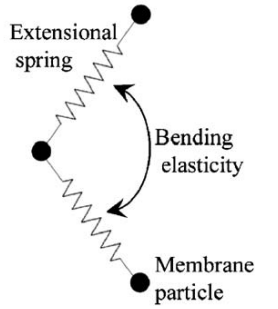
\includegraphics[width=0.2\linewidth]{mol3.png}
\caption{ Схема упругости при растяжении и изгибе между частицами в мембране~\cite{hosseini:2009}.}
\label{elasticity scheme}
\end{figure}

Для её описания используется четыре силы.
Первая сила возникает, когда стороны треугольников меняют свою длину.
$$
\vec {F_I}=k_I\left(1- \frac{l}{l_0}\right)\vec\tau,
$$
где $l$ -- длина ребра, $l_0$ -- равновесная длина, $k_I$ -- коэффициент жёсткости, $\vec {\tau}$ -- единичный вектор, 
направленный от одной вершины к другой.

К каждому узлу сходится несколько сторон, и каждая из них вносит свой вклад в общую силу F. 
Вторая сила определяется сжатием или расширением мембраны 
$$
{p_s}=k_s\left(1- \frac{s}{s_0}\right),
$$
где $s$ -- площадь треугольника, $s_0$ -- площадь равновесного треугольника, $k_s$ -- коэффициент расширения площади.

Третья сила пропорциональна изменению объема многогранника и прикладывается к вершинам треугольников в направлении, нормальном к поверхности 
$$
\vec{F_v}=k_v\left(1- \frac{v}{v_0}\right) s \vec{n},
$$
где $v$ -- объем многогранника, $v_0$ -- равновесный объем, $k_v$ -- коэффициент, $s$ -- площадь
треугольного элемента, а $n$ -- единичный нормальный вектор к этому треугольнику.

Четвёртая сила выражается через изгибающий момент~\cite{hosseini:2009} 
$$
 \vec{M_i}=k_M \tan\left(\frac{\theta}{2}\right)l \vec{\tau_i},
$$
где $\theta$ -- угол между соседними треугольными элементами, 
$k_m$ -- коэффициент жесткости, $\vec{\tau_i}$ -- единичный вектор, сонаправленный с общим краем двух треугольников 
и $l$ -- длина этой стороны.

Аналогичным образом могут быть смоделированы и другие клетки крови. Например, в отличие от эритроцитов, лейкоциты содержат ядро. 
Из-за этого они менее деформируемы, а их форма близка к сфере. Это влияет на их поведение в потоке крови.

Для определения параметров эритроцитов прибегают к методам численного моделирования~\cite{bessonov:2014}.

Фактически, можно легко указать на несколько недостатков данной модели. Например, рассмотрение всей клетки как однородной решетки 
делает невозможным учет любой органеллы в цитоплазме. Кроме того, эффективная упругость решетки зависит не только от 
пружинной постоянной, но и от конкретной формы, размера и топологии решетки. Это затрудняет сравнение между различными моделями 
и экспериментами. Более того, параметры модели на уровне частиц  модели не были систематически связаны с физиологическими измерениями; 
они должны принимать нереальные значения, чтобы предсказание было количественно сопоставимо с реальностью 


\subsection{Моделирование крови как неньютоновской жидкости}
Жидкость может считаться ньютоновской, если она удовлетворяет закону вязкости Ньютона, 
т.е. напряжение сдвига пропорционально скорости сдвига, а вязкость является константой пропорциональности, 
поэтому плазму крови, состоящую в основном из воды, можно считать ньютоновской. Однако у крови более сложные механические свойства. 
И мы предполагаем, что все макроскопические масштабы длины и времени достаточно велики по сравнению с масштабами длины и времени 
на уровне отдельного эритроцита. Таким образом, для упрощения построения модели и дальнейшей работы с ней можно рассматривать 
взвешенные клетки в плазме, как вязкую несжимаемую, неньютоновскую жидкость.

Такие методы применяется в тех сосудах, где клетки достаточно малы и многочисленны, чтобы их отдельную индивидуальность можно было
игнорировать, а их влияние на движение всей крови описывать усредненным способом. 
Так обстоит дело в крупных артериях (диаметр аорты, например, примерно в 2000 раз больше диаметра эритроцита). 
На практике эти методы применяются в изучении и моделировании сердечного выборса, печеночного кровотока, среднего артериального давления.

\textbf{Вязкость.}
Для начала рассмотрим простейшую конститутивную модель, основанную на предположении, что тензор дополнительных напряжений пропорционален
симметричной части градиента скорости.
$$
\tau=2\mu (\dot{\gamma})D,
$$
где $\tau $ -- тензор дополнительных напряжений, $D=(\nabla u+\nabla u^T)$ -- тензор скорости деформации, 
$\mu (\dot{\gamma})$ -- скорость сдвига.
Зависимость $\mu (\dot{\gamma})$ находят разными способами. Например, в~\cite{walburn:1976}, 
рассматривают зависимость вязкости от гематокрита и белка минус-альбумин: \\
$$
\mu (\dot{\gamma})=K{\gamma}^{n-1}, \qquad  K=C_1 \exp (C_2 H_t).
$$
Полученные таким способом результаты вязкости оказались схожи с результатами, которые были получены в~\cite{kim:2000} при помощи вязкозиметра.\\

\textbf{Вязкоупругость.}
Вязкоупругие жидкости -- это вязкие жидкости, обладающие способностью накапливать и высвобождать энергию. 
Упругая энергия объясняется свойствами мембраны РНК, демонстрирующей релаксацию~\cite{evans:1976} и зависящей от скорости сдвига.\\
Одной из простейших моделей, учитывающих вязкоупругость крови, является модель Максвелла~\cite{thurston:1972}:
$$
\tau+\lambda_1(\delta\tau / \delta t)=2\mu D,
$$  
где $\lambda_1$ -- время релаксации, a $\delta\tau / \delta t$ -- обобщение материальной производной по времени.
При построении данной модели полагают, что время релаксации зависит от скорости сдвига.
В~\cite{thurston:1994} данный метод используют для понимания неньютоновского вязкого характера крови после устойоявшегося поток.\\

\textbf{Предел текучести.}
Предел текучести обычно рассматривается как постоянное материальное свойство жидкости. 
Но зафиксированные пределы текучести имели большой разброс, который, стоит отметить, зависел от множества факторов.
Поэтому предел текучести стоит рассматривать не как константу, а как функцию времени и связанную с тиксотропией, 
как было предложено в~\cite{moller:2006}.
Более популярной моделью предела текучести является модель Кассона.
$$
\begin{aligned}
	&\sqrt{II_\tau} < \tau_Y\longrightarrow D=0 \\
	&\sqrt{II_\tau} \geq \tau_Y\longrightarrow
	\begin{cases}
		D   = \dfrac{1}{2\mu N}\left(1-\dfrac{\sqrt{\tau_Y}}{II_\tau}\right)^2\tau \\[10pt]
		\tau= 2\left(\sqrt{\mu N}+\dfrac{\sqrt{\tau_Y}}{\sqrt[4]{4II_D}}\right)^2
	\end{cases}
\end{aligned}
$$

В нашем случае предел текучести является параметра крови, например, для понимания, как будет вести себя кровь под влиянием какого-либо 
препарата, не станет ли она слишком вязкой или наоборот.
Однако, до сих пор использование предела текучести в качестве параметра моделирования крови остаётся спорным, 
в связи с неточностями его определения.

\subsection{Одномерные модели}

\textcolor{red}{В данном пункте мы осредняем все трёхмерные характеристики
по поперечному сечению и рассматриваем одномерную задачу.}

Привлекательность oдномерныx моделeй кровотока основана на разумных вычислительных затратах. 
Основные приложениями этих моделей являются транспорт газов крови и лекарств в организме, перераспределение кровотока при внешних 
или внутренних воздействиях, перераспределение кровотока в результате внутрисосудистых операций. Основными недостатками данных моделей 
являются сложность численных схем, высокая стоимость вычислений и спекулятивные граничные условия. 
Вычислительная область -- это сосудистая одномерная сеть человека или ее части. 
Сеть может быть создана на основе общих анатомических данных, таких как справочник анатомических карт~\cite{bunicheva:2013}, 
анатомические 3D модели или данные конкретного пациента.


Обозначим через $t$ -- время, через $x$ -- координату вдоль сосуда, через$A(t, x)$ -- площадь поперечного сечения сосуда, 
$u(t, x)$ и $p$ -- усредненную по сечению линейную скорость и трансмуральное давление крови. Баланс массы и импульса в переменных 
$(A, u, p)$ соответствует уравнениям
\begin{align}
    \label{eq:mass-balance}
    f_A=&\frac{\partial A}{\partial t}+\frac{\partial Au}{\partial x},\\
    \label{eq:momentum-balance}
    f_u=&\frac{\partial u}{\partial t}+ \frac{\partial u^2/2+p/\rho}{\partial x}
\end{align}

Правые части уравнений (масса источника или поглотителя на единицу длины, ускорение) зависят от моделируемого процесса. 
Эта модель была использована в~\cite{bunicheva:2004} для моделирования воздействия гравитационной перегрузки на системное кровообращение. 

В одномерных моделях кровотока традиционное описание упругих свойств стенки сосуда обеспечивается отношением давления к площади 
поперечного сечения $P(A)$. Прямой подход к получению отношения $P(A)$ является точное одновременное измерение в естественных 
условиях давления и площади в разные моменты времени. Но, как можно понять, такой метод не всегда удобен в реальности.

Качественный анализ физических экспериментов подтверждает, что функция $P(A)$ должна быть монотонной S-подобной кривой. 
Такая кривая удовлетворительно описывает  состояния как круглого, так и эллиптического сечения. 
На практике S-подобная зависимость давления от площади часто аппроксимируется аналитической функцией. 

\begin{figure}[h]
\centering
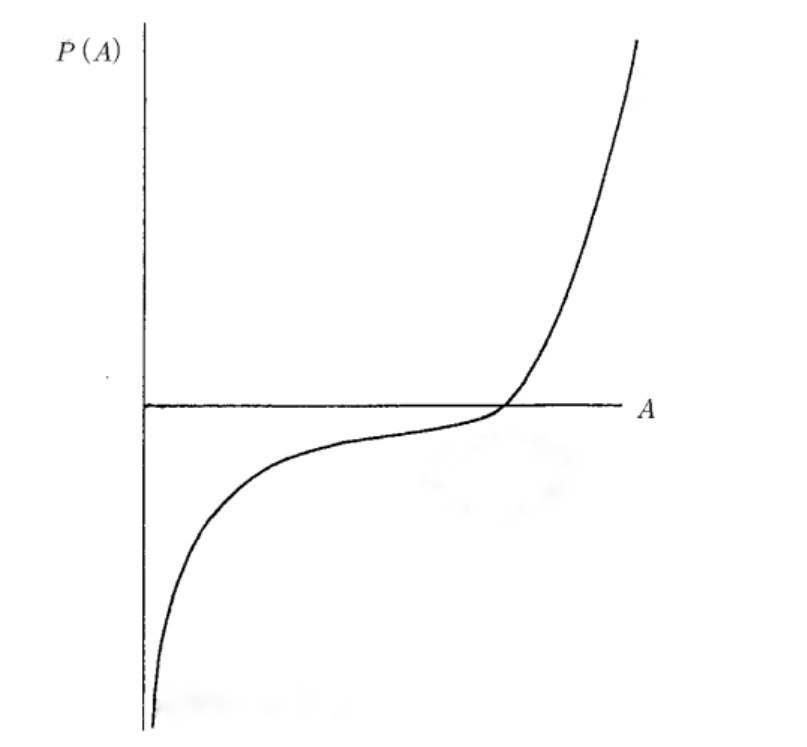
\includegraphics[width=0.3\linewidth]{IMG_20230309_021324_943-01.jpeg}
\caption{ График зависимости $P(A)$~\cite{pedly:1998}.}
\label{fig:mpr}
\end{figure}

Правильные упругие свойства артерий и вен могут быть описаны следующей функцией~\cite{holodov:2001}:
\begin{equation}
    \label{eq:elastic-propeties}
    P(A)=\rho c^2_0 f(a/a_0), 
    \quad
    f(k)=\begin{cases}
    \exp(k-1)-1, &k>1 \\ \ln(k), &k \leq 1
    \end{cases}
\end{equation}

Для каждого k-го сосуда известны законы сохранения массы и импульса(\ref{eq:mass-conserv}),(\ref{eq:mom-conserv}). 
И для замыкания системы уравнений необходимо учесть уравнение состояния описывающее изменение поперечного сечения сосуда в зависимости 
от трансмурального давления(\ref{eq:t-pressure}).
\begin{align}
    \label{eq:mass-conserv}
    \frac{\partial S_k}{ \partial t} + \frac{\partial(u_kS_k)}{\partial x}&=\varphi _k(t,x,S_k,u_k,r_i),\\
    \label{eq:mom-conserv}
    \frac{\partial u_k}{\partial t} + \frac{\partial(u_k^2/2+p_k/\rho_k)}{\partial x}&= \psi_k(t,x,S_k,u_k,r_i),\\
    \label{eq:t-pressure}
    p_k(t,x)-p_*(t,x)&=\rho_k c^2_{k0}f_k(S_k(t,x)),
\end{align}
где $t$ -- время, $x$ -- расстояние вдоль сосуда, $\rho$=const -- плотность, $c_{k0}(t,x)$ -- скорость распространения малых возмущений,
  $p_k(t,x)$ -- давление внутри сосуда (от атмосферного) $p_*(t,x)$ -- избыточное давление в тканях, окружающих сосуд, 
  $S_ku_k=Q(t,x)$ -- массовый расход, $\varphi _k(t,x,S_k,u_k,r_i)$ -- источник/утечка массы, $\psi_k(t,x,S_k,u_k,r_i)$ -- внечние силы (гравитация, трение и т.~д.),
  $k=1,2,\ldots$ -- индекс сосуда.
\\ 
Другие обобщения модели эластичной стенки сосуда являются модели вязкоупругой стенки. В таких моделях зависимость 
$
P(A)=F(A,\partial {A} / \partial {t},\partial^2{A} / \partial {t^2},\partial^2{A} / \partial {x^2})
$.

{\bf Граничные условия.}
Для одномерных моделей кровотока необходимы граничные условия на стыках сосудов, входах и выходах в сети сосудов. 
Для всех сосудов граничные условия должны включать условия совместимости по характеристикам гиперболических уравнений(\ref{eq:mass-balance}), (\ref{eq:momentum-balance}).
В каждой конечной точке сосуда требуется только одно дополнительное условие совместимости.
Вторым условным граничным условием на стыке N сосудов является сохранение массы:
\begin{equation}
    \label{eq:conserv-mass}
    \sum_{k=k_1,k_2,...,k_N} \varepsilon_k A_k(t,x_k)u_k(t,x_k)=0,
\end{equation}
где {$k_1,...,k_N$} -- индексы сосудов, $\varepsilon_k=1, x_k=0$ -- для входящих сосудов, 
$\varepsilon_k=1, x_k=L_k$ -- для выходящих сосудов.

Другими граничными условиями является $N$ условий перепада давления:
\begin{equation}
    \label{eq:p-pressure}
    p_k\left(A_k\left(t,x_k\right)\right)-p^l(t)=\varepsilon_k R^l_k A_k(t,x_k)u_k(t,x_k)
\end{equation}
или $N$ интегральных условий сохранения Бернулли выражающих непрерывность полного давления:
\begin{equation}
    \label{eq:bernulli}
    \frac{u^2_k}{2}+\frac{p_k(A_k)}{\rho}=P^l,
\end{equation}
где $p^l$ и $P^l$ -- давление и полное давление в точке с индексом $l$, соответсвенно.

Подводя итог, можно сказать, что на каждом пересечении сосудов накладывается $2N + 1 $ граничных условий в виде 
нелинейных алгебраических уравнений, которые могут быть эффективно сведены к $N + 1$ нелинейным уравнениям.

Выходы сети артерий и входы сети вен должны быть связаны с множеством мелких неучтенных сосудов, относящихся к микрососудистым регионам.
 Поток в таких сосудах не может быть описан одномерными моделями течения (\ref{eq:mass-balance})-(\ref{eq:mass-conserv}) 
 из-за большого количества сосудов, сложной структуры микрососудистых сетей и неньютоновской реологии крови.

Более простой подход заключается в том, чтобы объединить артерий и вены в точки соединения, 
где выполняются (\ref{eq:conserv-mass}),(\ref{eq:p-pressure}). Коэффициенты сопротивления $ R^l_k$ оцениваются  по известному перепаду 
давления между артериями и венами. Чем больше сосудистая сеть, тем меньше сосудов объединяются, тем выше точность метода. 
Более подходящие граничные условия оттока: отдельные участки мелких артерий и микроциркуляции моделируются как структурированные деревья, 
чей импеданс корней может быть оценен из линеаризации управляющих уравнений.

Многие авторы~\cite{alastruey:2008} выполняют сопряжение во временной области 1D моделей кровотока с электрическими цепями 
(единичными параметрами) 0D моделей. 0D модели обеспечивают корректные граничные условия для глобальных моделей кровотока.
\\

{\bf Численные схемы.}
С математической точки зрения, одномерная модель кровотока представляет собой алгебраическо-дифференциальную систему, 
состоящую из набора гиперболических уравнений в сосудах и набора алгебраических уравнений на стыках и входах/выходах сети сосудов. 
Дробные временные шаги неявно-явных схем разделяют вычисления на отдельные локализованные части и поэтому легко распараллеливаются.

Мы рассматриваем системный круг, представленный двумя связанными сетями артерий и вен (см.Рис.~\ref{ss}). 
Сосудистая система состоит из 341 сосуда с анатомически адекватными свойствами (длина, диаметр, упругие свойства), вен и артерий. 
Вены и артерии соединены в 162 точках, на которые наложены граничные условия (\ref{eq:conserv-mass}),(\ref{eq:p-pressure}). 

\begin{figure}[h]
\centering
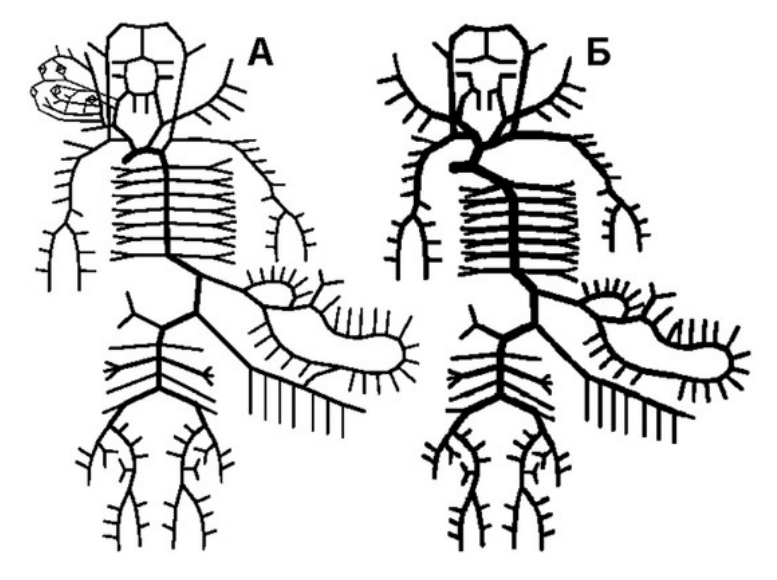
\includegraphics[width=0.5\linewidth]{krug.png}
\caption{Упрощённая структура сосудов системного круга. А—артерии, Б—вены.}
\label{ss}
\end{figure}

В каждом сосуде мы вводим одномерную равномерную сетку и дискретизируем систему (\ref{eq:mass-balance}),(\ref{eq:momentum-balance}) 
методом монотонных характеристик первого порядка. Уравнения расширяются набором жестких ОДЕ, которые описывают работу сердца в терминах 
усредненной по объему модели.

Система жестких ОДУ, решаемая неявным методом Рунге-Кутта третьего порядка, обеспечивает граничные условия на входе и выходе сердца. 
Алгебраическая дифференциальная система (\ref{eq:mass-balance}),(\ref{eq:momentum-balance}), (\ref{eq:conserv-mass}),(\ref{eq:p-pressure}) 
в сочетании с зависимостью давления от площади и соответствующими граничными условиями на входе и выходе сердца 
и микроциркуляторных областях, решается по схеме с дробным шагом по времени схема, которая разделяет вычисления на 
локальные независимые части (отдельные сосуды и отдельные точки соединения).

На гиперболическом подэтапе мы применяем явный метод характеристик для каждого сосуда и контролируем шаг по времени с помощью 
ограничения устойчивости $\tau = 0.9 s_{\max}$, $s_{\max}=\max_{k,i}|\lambda _{k,i}|/h_k$, где $h_k$ -- размер сетки в сосуде $k$, 
$\lambda$ -- размер сетки в сосуде $k$,  $\lambda _{k,i}$ -- наибольшее (по величине) собственное значение якобиана для  (\ref{eq:mass-balance}),(\ref{eq:momentum-balance}), 
 в точке сетки.

В алгебраическом подэтапе мы применяем метод Ньютона для системы уравнений в каждом узле пересечения. 
Система состоит из уравнений (\ref{eq:conserv-mass}),(\ref{eq:p-pressure}) и условие совместимости по характеристикам (\ref{eq:mass-balance}),(\ref{eq:momentum-balance}). 
Влияние атеросклеротической бляшки учитывается в модели эластичной стенки. Здоровые сосуды описываются уравнением (\ref{eq:elastic-propeties}), 
обеспечивающим достоверную корреляцию с экспериментальными кривыми. Атеросклеротические артерии рассматриваются как 
трехслойные цилиндрические оболочки, деформированные внутренним давлением крови. Внутренний и внешний слои оболочки -- это 
фиброзная крышка и стенка артерии, соответственно. Деформации фиброзной пробки и стенки сосуда моделируются с помощью 
волоконно-эластичной модели. В простейшей версии волоконной осесимметричной модели оболочка представлена набором кольцевых волокон, 
которые сопротивляются только растяжению и сжатию волокон, как неогуковские материалы.

\begin{equation}
    \label{loc-force}
    \vec{F}=\frac{\partial}{\partial s}(T\vec{\tau}),
    \quad
    T=\mu\left(\left|\frac{\partial \vec{X}}{\partial s}\right|^2-\left|\frac{\partial \Vec{X}}{\partial s}\right|^{-2}\right).
\end{equation}
Здесь $\mathbf{F}$ обозначает плотность локальной силы, $T(s)$ обозначает натяжение волокна, 
$\Vec{\tau} =\partial \Vec{X}/\partial s^{-1}$ единичный касательный вектор, $\Vec{X}(s)$ 
представляет собой положение точек волокна в пространстве, координата Лагранжа s -- длина дуги волокна в ненапряженном состоянии. 
Липидный пул (промежуточная оболочка) имитируется набором радиальных пружин с нелинейной зависимостью между силой реакции и смещением

Отношение давления к площади атеросклеротической артерии получено из предположения о статическом равновесии стенки: 
внутреннее давление крови уравновешивается упругими силами вышеупомянутой системы волоконных пружин, возникающими при ее смещении. 
На основе смещений можно рассчитать поперечную площадь сечения $A$ как реакцию на любое давление крови. 
Восстановление равновесного состояния получено в рамках его численной аппроксимации: конечно-разностная дискретизация (\ref{loc-force}) 
приводит к системе нелинейных алгебраических уравнений, которая должна быть решена итерационно методом Ньютона.

Численная модель <<волокно-пружина>> имеет преимущества прямые обобщения с другими типами волокон и, таким образом, 
может быть распространена на гораздо более широкий класс геометрий бляшек.

\begin{figure}[h]
\centering
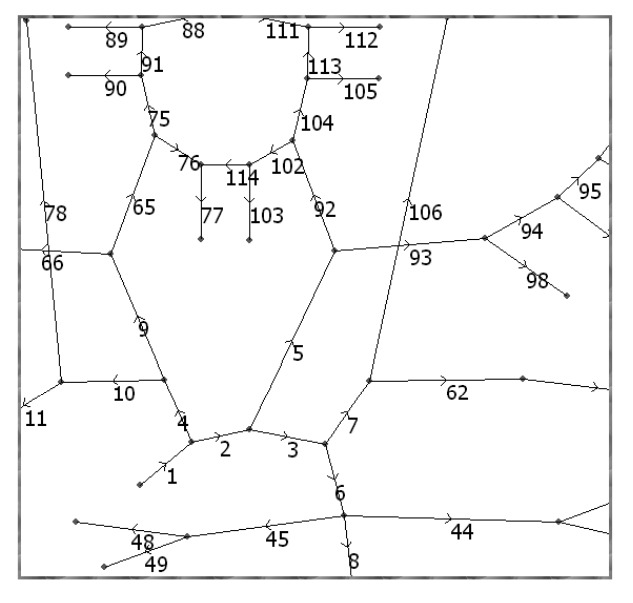
\includegraphics[width=0.4\linewidth]{chast.png}
\caption{Участок сосудов системного круга.}
\label{ych}
\end{figure}

В эксперименте мы предполагаем, что левая общая сонная артерия (№5 на Рис.\ref{ych}) повреждена протяженной атеросклеротической бляшкой 
с просветом 10\%, 30\%, 50\% и 100\%. Коэффициенты упругой бляшки взяты из~\cite{vassilevski:2011}. 
Профили скоростей в наружном сонном продолжении (№94) и артериях круга Уиллиса (№104, 102) показаны на Рис.~\ref{sc}. 
Наиболее заметные изменения в скорости происходят в случае бляшек с просветом 30\% и 10\%. 
В малой артерии Виллисова круга (№104) и на продолжении левой наружной сонной артерии (№94) наблюдается значительное снижение скорости крови.

\begin{figure}[h]
\centering
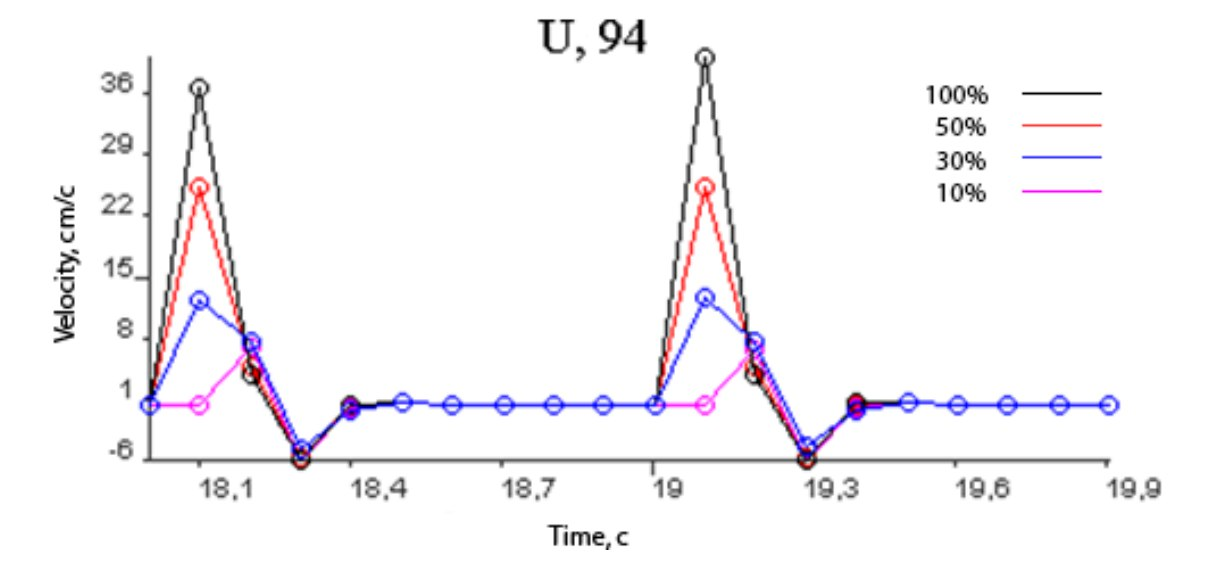
\includegraphics[width=0.45\linewidth]{94.jpg}
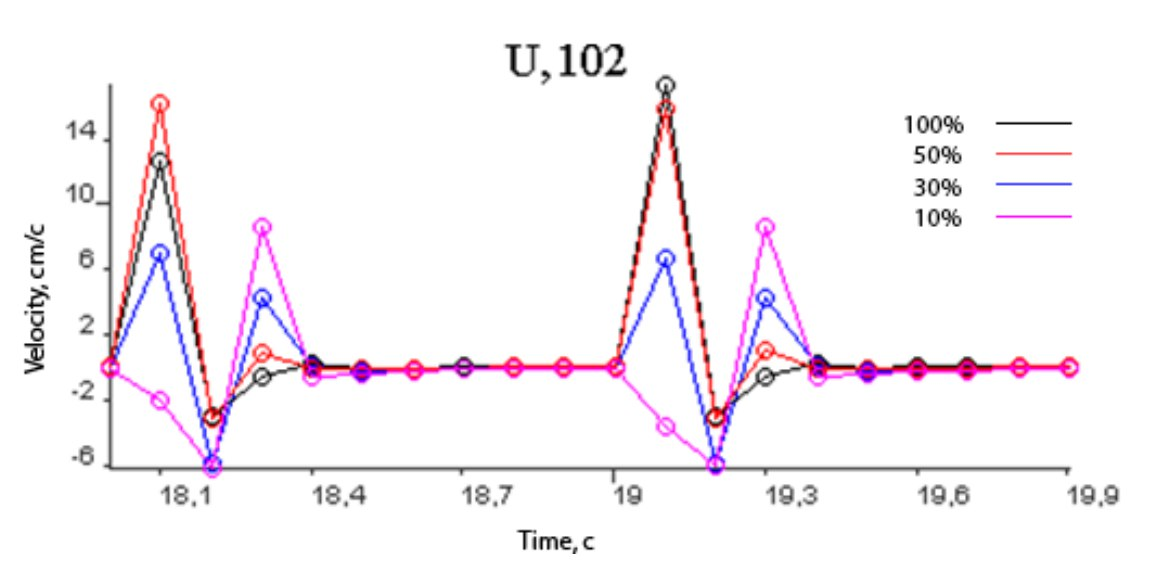
\includegraphics[width=0.45\linewidth]{102.jpg}\\
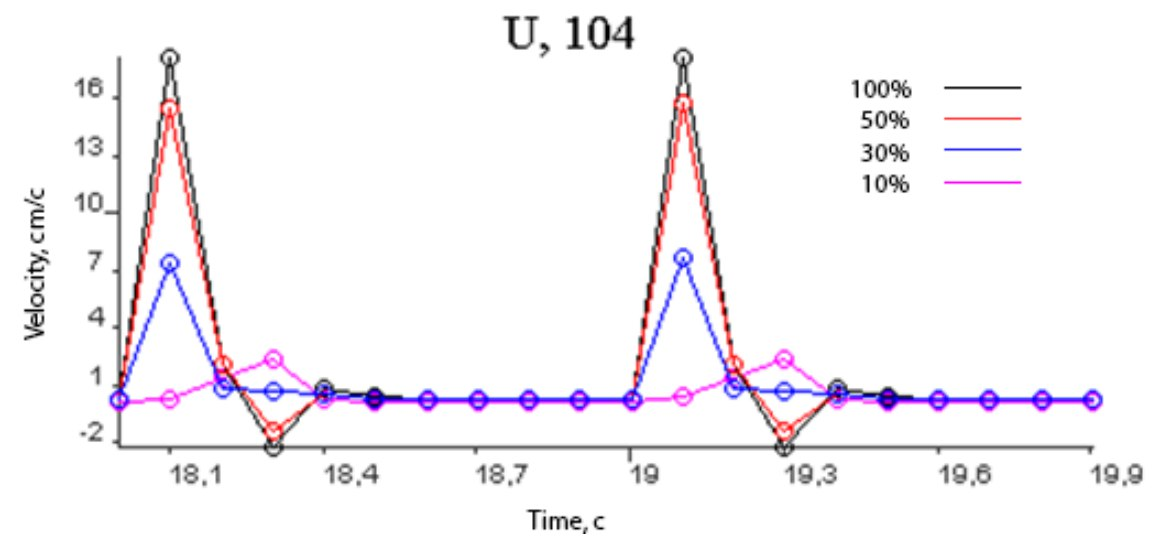
\includegraphics[width=0.45\linewidth]{104.jpg}
\caption{Скорость (см/с) в сосудах 94, 102, 104 для различных просветов. Здоровый сосуд
соответствует 100\% просвету}
\label{sc}
\end{figure}


\section{Вычислительный эксперимент}
\subsection*{Задача бегущей волны}

Задача бегущей волны - это численный метод решения задач распространения волны. Данный метод основывается на дискретизации 
времени и пространства. Мы разбиваем области на конечное число участков определённой длины и вычисляем значение функции в каждом узле.
Для решения данной задачи будем использовать метод конечных разностей.

Имеем систему уравнений:

\begin{equation*}
    \label{sys_of_eq}
    \begin{cases}
        &\frac{\partial A}{\partial t}+\frac{\partial Au}{\partial x}=0\\
        &\frac{\partial u}{\partial t}+U\frac{\partial u}{\partial x}+\frac{1}{\rho}\frac{\partial p}{\partial x}=\frac{f}{\rho A}\\
        &f=-2(\xi+2)\mu\pi U\\
        &p=\frac{4}{3}\sqrt{\pi}\frac{Eh}{A_0}(\sqrt{A}-\sqrt{A_0})
    \end{cases}.
\end{equation*}

Для работы с этой системой необходимо произвести обезразмеривание. Это необходимо, чтобы избавиться от размерности величин,
следовательно сделать систему удобнее для моделирования и уменьшить количество задаваемых переменных, 
а так же иметь возможность сравнивать результаты и выводить закономерности

Разделим уравнение на ${U_0 t_0}/{x_0}=1$,  причём $t_0$ находим из граничных условий, 
$x_0$ из геометрических характеристик, а $A_0$ из начальных условий/состояния покоя. Получается более понятная система:

\begin{equation}
    \label{sys_of_eq1}
    \begin{cases}
        \frac{\partial A}{\partial t}+\frac{\partial Au}{\partial x}=0\\
        \frac{\partial u}{\partial t}+\frac{1}{2}\frac{\partial u^2}{\partial x}-\frac{\partial p}{\partial x}+M_f \frac{u}{A}=0\\
        p=M_p(\sqrt{A}-1).
    \end{cases},
    \end{equation}
где 
$$ M_f=\frac{-2(\xi+2)\mu \pi t_0}{\rho A_0},\quad  M_P=\frac{\frac{4}{3}\sqrt{\pi}Eh}{\rho U_0\sqrt{A_0}}(\sqrt{A}-1).$$



Как уже говорилось, систему будем решать методом конечных разностей. Представим первое уравнение в виде:
$$
\begin{aligned}
    &\frac{\hat{A_i}-A_i}{\tau}+\frac{F_{i+1/2}-F_{i-1/2}}{h}=0,\\
    &F_{i+1/2}=\begin{cases}
        u_i A_i, &u_i>0\\
        u_{i+1}A_{i+1},& u_i<0
    \end{cases}.
\end{aligned}
$$
А для второго уравнения полагаем, что $Q(t)$ нам дан, а давление на границе нулевое, т.е. 

$
\begin{aligned} 
    p=M_p(\sqrt{A}-1)=0\longrightarrow A=1, \quad
    Q=uA \longrightarrow
    Q=u.
\end{aligned}
$

Второе уравнение будет выглядеть следующим образом:

$$
\begin{aligned}
    &\frac{\hat{u_i}-u_i}{\tau}+\frac{F_{i+1/2}^u-F_{i-1/2}^u}{h}+\frac{\partial P}{\partial x}+M_P\frac{\hat{u_i}}{\hat{A_i}}=0,\\
    &F_{i+1/2}^u=\begin{cases}
        \frac{u_i^2}{2}, &u_i>0\\
        \frac{u_{i+1}^2}{2}, &u_i<0
    \end{cases}.
\end{aligned}
$$



\subsection*{TVD-схема}
Схема TVD используется для численного решения уравнений гидродинамики. Она работает по следующему принципу.
Задаётся распределение параметров в начальный момент времени. 
Затем с помощью конечно-разностной схемы вычисляются значения параметров в каждый последующий момент времени. 
При этом схема TVD обеспечивает сохранение свойства "total variation diminishing", т.е. сумма изменений параметров 
на каждом шаге не увеличивается по сравнению с предыдущим шагом. А так же сохраняет высокий порядок точности и является консервативной.

Для обеспечения всех свойств схемы используются ограничители. Они ограничивают распространение возмущений, уменьшают ошибки при
аппроксимации и повышают устойчивость метода. 
Для каждого типа задач есть более или менее подходящие ограничители. Для задачи бегущей волны можно рассмотреть ограничители:
MinMod, MC, Van Leer, SuperBee, Umist, Ospre.
Задаются они следующим образом:

MinMod: $
\begin{aligned}
	\phi(r)=\begin{cases}
        0, &r\leq 0\\
        r, &0<r\leq 1\\
        1, &r>1
    \end{cases}
\end{aligned}
$


MC:$
\begin{aligned}
     \phi(r)=\begin{cases}
        0, &r\leq0\\
        2r, &0<r\leq\frac{1}{3}\\
        \frac{1+r}{2}, &r\leq3\\
        2, &r>3
    \end{cases}
\end{aligned}
$ 


VanLeer:$
\begin{aligned}
    \phi(r)=\frac{r+|r|}{1+|r|}
\end{aligned}
$


SuperBee: $
\begin{aligned}
    \phi(r)=\begin{cases}
        0, &r\leq 0\\
        2r, &0<r\leq 0.5\\
        1, &0.5<r\leq 1\\
        r, &1<r\leq 2\\
        2, &r>2
    \end{cases}
\end{aligned}
$


Umist: $
\begin{aligned}
    \phi(r)=\begin{cases}
        0, &r\leq 0\\
        2r, &0<r\leq 0.2\\
        0.52+0.75r, &0.2<r\leq \frac{3}{7}\\
        0.75+0.25r, &\frac{3}{7}<r\leq \frac{7}{3}\\
        2, &r>\frac{7}{3}
    \end{cases}
\end{aligned}
$


Ospre: $
\begin{aligned}
   \phi(r)=
    \frac{1.5(r^2+r)}{r^2+r+1}
\end{aligned}
$


На основе описанного выше можно произвести расчёты и построить графики распределения объема по времени, а так же сравнить
заданные ограничители.

\begin{figure}[h!]
    \centering
    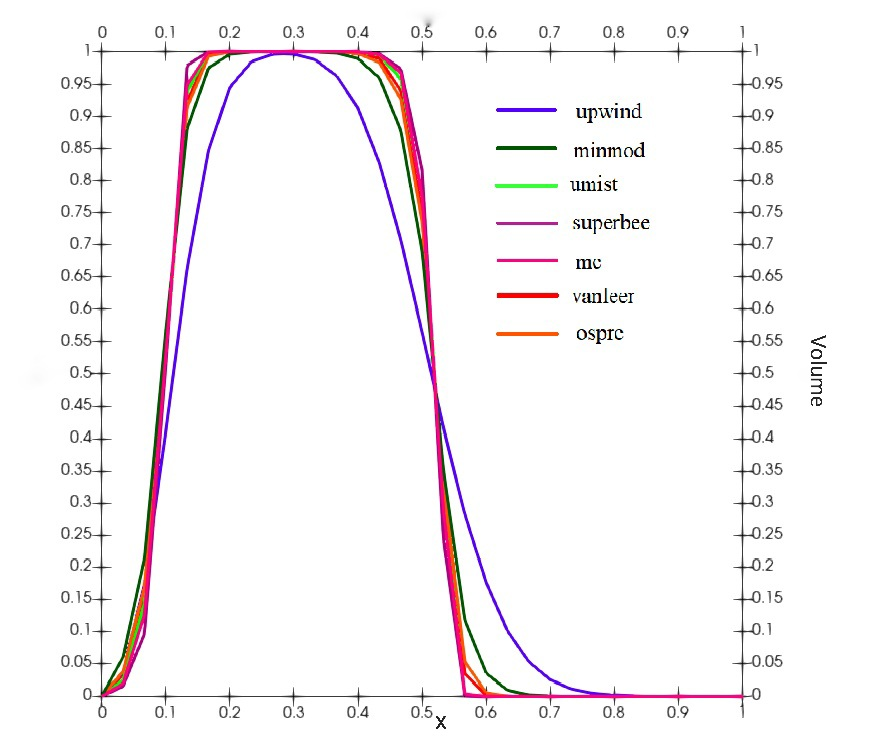
\includegraphics[width=0.6\linewidth]{0.3.jpeg}
    \caption{Распределение объёма в момент 0.3}
    \label{03}
\end{figure}

\begin{figure}[h!]
    \centering
     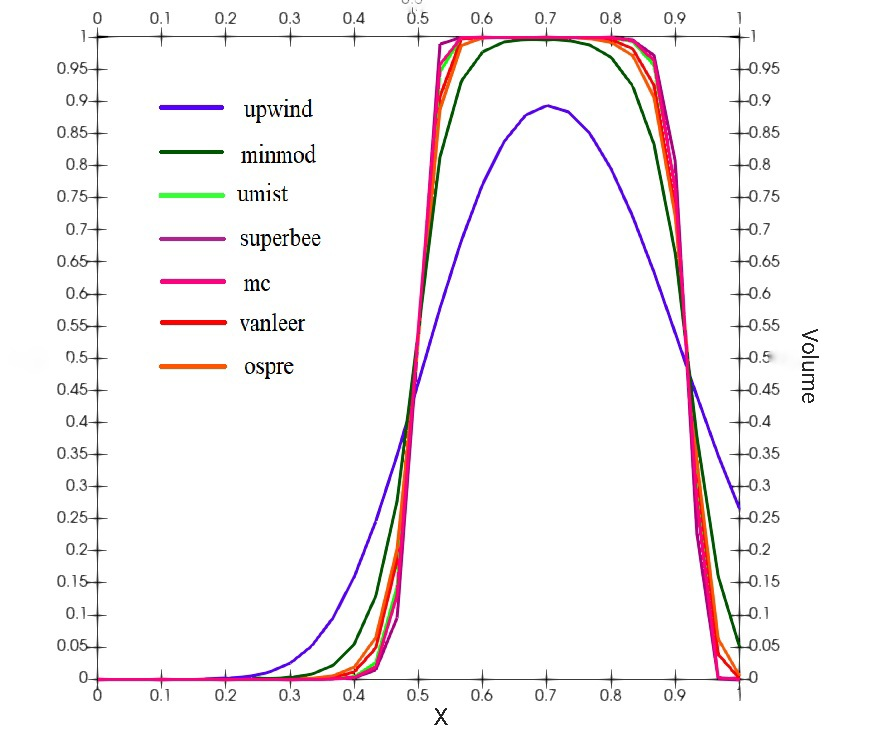
\includegraphics[width=0.6\linewidth]{0.7.jpeg}
    \caption{Распределение объёма в момент 0.7}
    \label{07}
\end{figure}


Погрешности ограничителей:
\begin{figure}[h!]
    \centering
     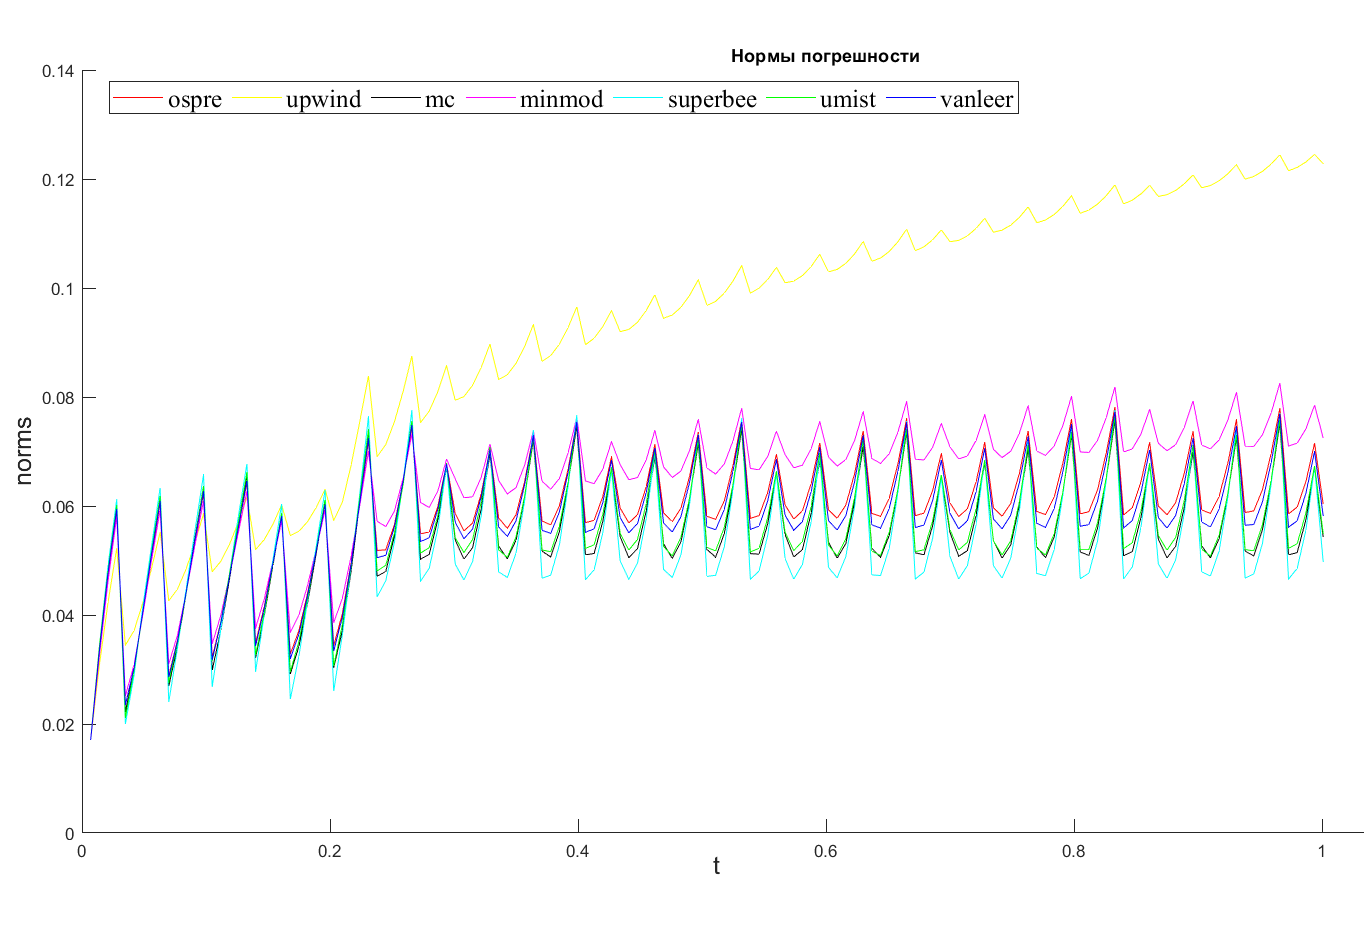
\includegraphics[width=1\linewidth]{norm.png}
    \caption{График погрешностей.}
    \label{norms}
\end{figure}

\begin{table}[tp!]
\centering
\caption {Значения погрешностей в момент 0.56.}
\label{tab:norms}
\begin{tabular}{|l|l|c|c|c|c|c|c|c|c|}
\hline
Ограничитель & Значение \\
\hline
SuperBee & 0.0659053\\
\hline
MC &  0.0659238\\
\hline
Umist & 0.0663728\\
\hline
Van Leer & 0.0685166\\
\hline
Ospre &  0.069493\\
\hline
MinMod & 0.0737164\\
\hline
Upwind  & 0.103783\\
\hline
\end{tabular}
\end{table}


На основе полученных данных можем сделать вывод, что для моделирования данной задачи не стоит использовать такие ограничители, как
Upwind и MinMod, а самыми точными оказались SuperBee и MC
\section{Примеры расчётов кровотока}
\subsection{Расчёт полной системы циркуляции}
Для примера применения одномерной модели кровотока для расчёта полной системы циркуляции рассмотрим
задачу о влиянии атеросклеротической бляшки на параметры течения крови, изученной в работе \cite{vassilevski:2011}.

На первом этапе решения задачи строится граф, описывающий изучаемую циркуляционную систему.
Он представленный двумя связанными сетями артерий и вен (см. Рис.~\ref{ss}). 
Сосудистая система состоит из 341 сосуда с анатомически адекватными свойствами (длина, диаметр, упругие свойства), вен и артерий. 
Вены и артерии соединены в 162 точках, на которые наложены граничные условия (\ref{eq:conserv-mass}),(\ref{eq:p-pressure}). 

\begin{figure}[h]
\centering
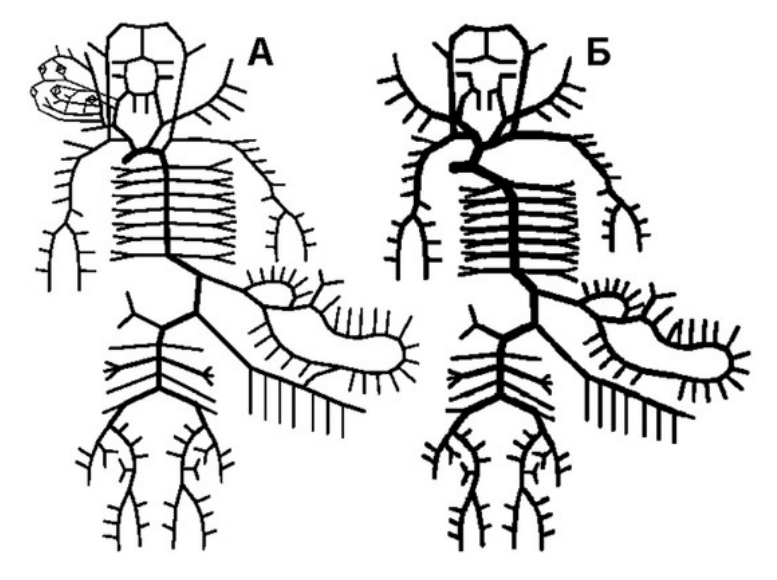
\includegraphics[width=0.5\linewidth]{krug.png}
\caption{Упрощённая структура сосудов системного круга. А—артерии, Б—вены.}
\label{ss}
\end{figure}

Далее в каждом сосуде вводится одномерную равномерную сетку и дискретизируем систему (\ref{eq:mass-balance}),(\ref{eq:momentum-balance}) 
методом монотонных характеристик первого порядка. Уравнения расширяются набором жестких ОДЕ, которые описывают работу сердца в терминах 
усредненной по объему модели.

Система жестких ОДУ, решаемая неявным методом Рунге-Кутта третьего порядка, обеспечивает граничные условия на входе и выходе сердца. 
Алгебраическая дифференциальная система (\ref{eq:mass-balance}),(\ref{eq:momentum-balance}), (\ref{eq:conserv-mass}),(\ref{eq:p-pressure}) 
в сочетании с зависимостью давления от площади и соответствующими граничными условиями на входе и выходе сердца 
и микроциркуляторных областях, решается по схеме с дробным шагом по времени схема, которая разделяет вычисления на 
локальные независимые части (отдельные сосуды и отдельные точки соединения).

На гиперболическом подэтапе применяется явный метод характеристик для каждого сосуда и контролируем шаг по времени с помощью 
ограничения устойчивости $\tau = 0.9 s_{\max}$, $s_{\max}=\max_{k,i}|\lambda _{k,i}|/h_k$, где $h_k$ -- размер сетки в сосуде $k$, 
$\lambda$ -- размер сетки в сосуде $k$,  $\lambda _{k,i}$ -- наибольшее (по величине) собственное значение якобиана для  (\ref{eq:mass-balance}),(\ref{eq:momentum-balance}), 
 в точке сетки.

В алгебраическом подэтапе применяется метод Ньютона для системы уравнений в каждом узле пересечения. 
Система состоит из уравнений (\ref{eq:conserv-mass}),(\ref{eq:p-pressure}) и условие совместимости по характеристикам (\ref{eq:mass-balance}),(\ref{eq:momentum-balance}). 
Влияние атеросклеротической бляшки учитывается в модели эластичной стенки. Здоровые сосуды описываются уравнением (\ref{eq:elastic-propeties}), 
обеспечивающим достоверную корреляцию с экспериментальными кривыми. Атеросклеротические артерии рассматриваются как 
трехслойные цилиндрические оболочки, деформированные внутренним давлением крови. Внутренний и внешний слои оболочки -- это 
фиброзная крышка и стенка артерии, соответственно. Деформации фиброзной пробки и стенки сосуда моделируются с помощью 
волоконно-эластичной модели. В простейшей версии волоконной осесимметричной модели оболочка представлена набором кольцевых волокон, 
которые сопротивляются только растяжению и сжатию волокон, как неогуковские материалы.

\begin{equation}
    \label{loc-force}
    \vec{F}=\frac{\partial}{\partial s}(T\vec{\tau}),
    \quad
    T=\mu\left(\left|\frac{\partial \vec{X}}{\partial s}\right|^2-\left|\frac{\partial \Vec{X}}{\partial s}\right|^{-2}\right).
\end{equation}
Здесь $\mathbf{F}$ обозначает плотность локальной силы, $T(s)$ обозначает натяжение волокна, 
$\Vec{\tau} =\partial \Vec{X}/\partial s^{-1}$ единичный касательный вектор, $\Vec{X}(s)$ 
представляет собой положение точек волокна в пространстве, координата Лагранжа s -- длина дуги волокна в ненапряженном состоянии. 
Липидный пул (промежуточная оболочка) имитируется набором радиальных пружин с нелинейной зависимостью между силой реакции и смещением

\begin{figure}[h]
\centering
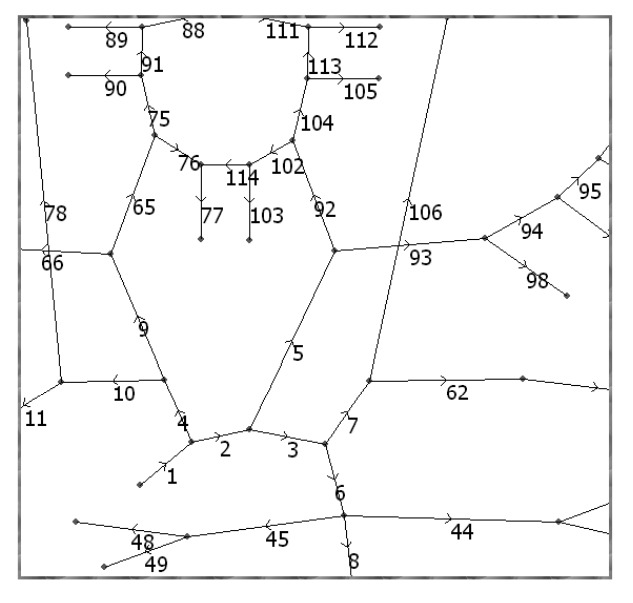
\includegraphics[width=0.4\linewidth]{chast.png}
\caption{Участок сосудов системного круга.}
\label{ych}
\end{figure}

\begin{figure}[h!]
\centering
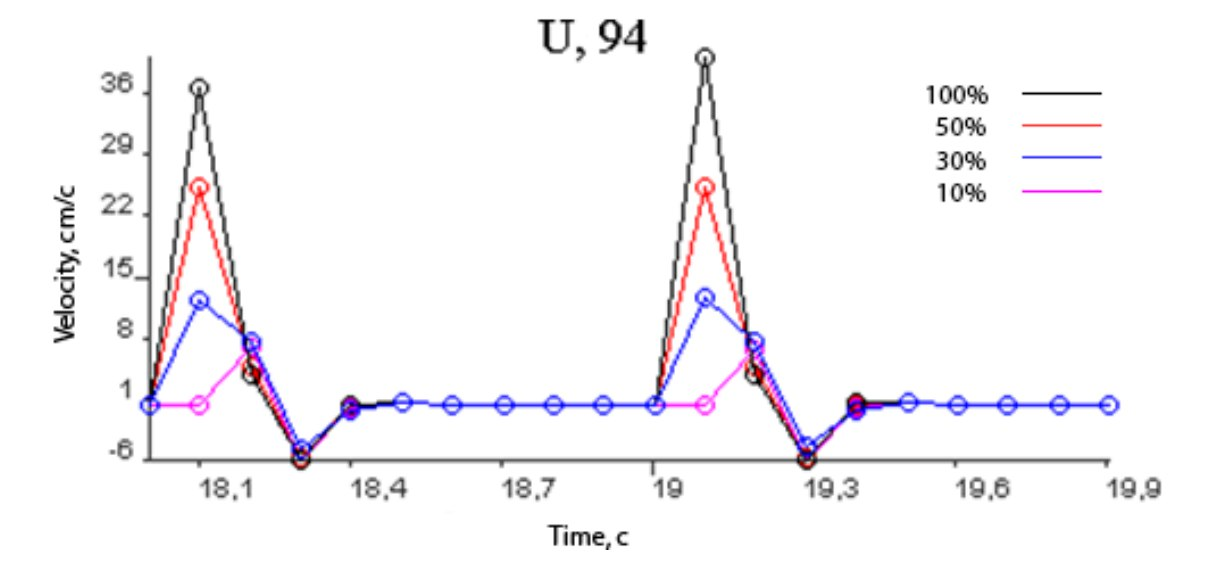
\includegraphics[width=0.45\linewidth]{94.jpg}
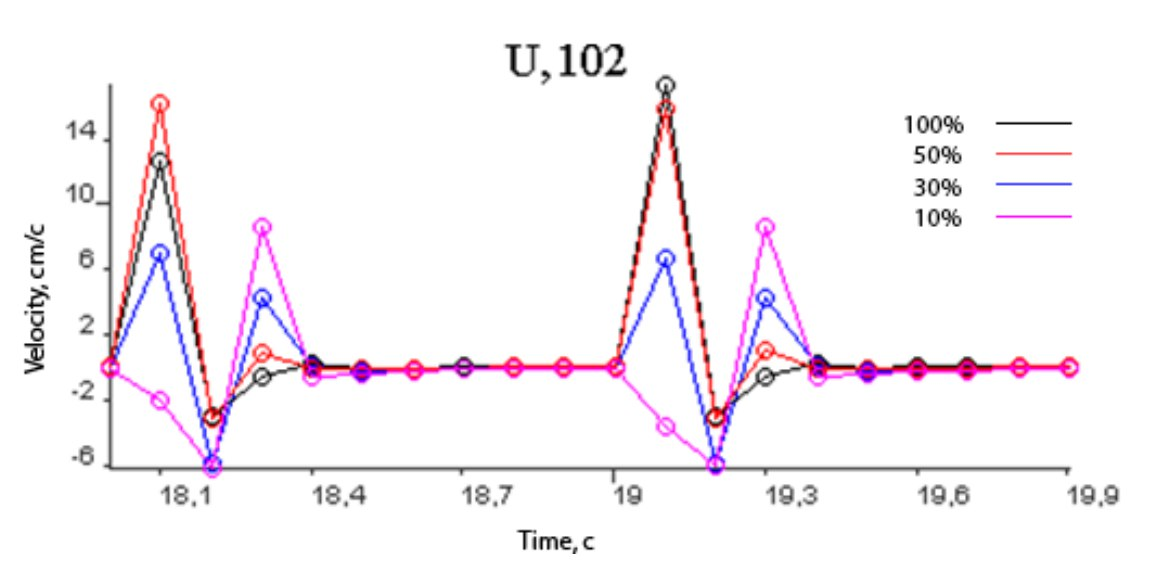
\includegraphics[width=0.45\linewidth]{102.jpg}\\
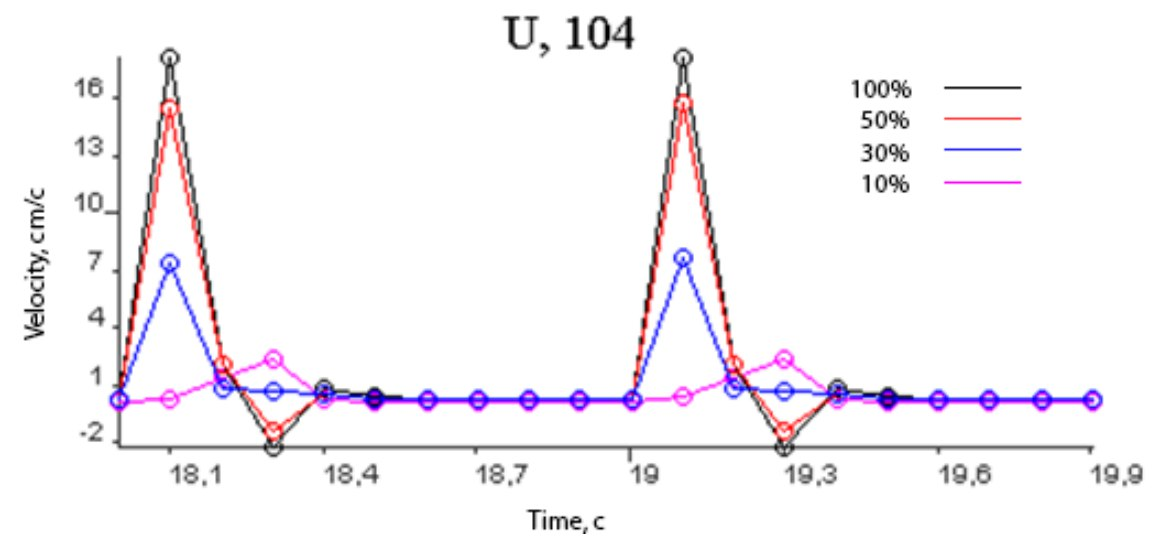
\includegraphics[width=0.45\linewidth]{104.jpg}
\caption{Скорость (см/с) в сосудах 94, 102, 104 для различных просветов. Здоровый сосуд
соответствует 100\% просвету}
\label{sc}
\end{figure}

Отношение давления к площади атеросклеротической артерии получено из предположения о статическом равновесии стенки: 
внутреннее давление крови уравновешивается упругими силами вышеупомянутой системы волоконных пружин, возникающими при ее смещении. 
На основе смещений можно рассчитать поперечную площадь сечения $A$ как реакцию на любое давление крови. 
Восстановление равновесного состояния получено в рамках его численной аппроксимации: конечно-разностная дискретизация (\ref{loc-force}) 
приводит к системе нелинейных алгебраических уравнений, которая должна быть решена итерационно методом Ньютона.

Численная модель <<волокно-пружина>> имеет преимущества прямые обобщения с другими типами волокон и, таким образом, 
может быть распространена на гораздо более широкий класс геометрий бляшек.

В численном эксперименте предполагается, что левая общая сонная артерия (№5 на Рис.\ref{ych}) повреждена протяженной атеросклеротической бляшкой 
с просветом 10\%, 30\%, 50\% и 100\%. Коэффициенты упругой бляшки взяты из~\cite{vassilevski:2011}. 
Профили скоростей в наружном сонном продолжении (№94) и артериях круга Виллиса (№104, 102) показаны на Рис.~\ref{sc}. 
Наиболее заметные изменения в скорости происходят в случае бляшек с просветом 30\% и 10\%. 
В малой артерии Виллисова круга (№104) и на продолжении левой наружной сонной артерии (№94) наблюдается значительное снижение скорости крови.


\subsection{Расчётная схема для моделирования течения в сосуде по одномерной модели}
Рассмотрим систему уравнений, описывающую кровоток в одиночном сосуде (\ref{eq:mass-conserv}) -- (\ref{eq:mom-conserv}) при условии
отсутствия источников/стоков ($\varphi=0$).
Из внешних сил, действующих на поток будем учитывать силу трения.
Для этого зададимся профилем скорости согласно \cite{smith:2002}:
$$
\tilde u(x, \xi) = u(x) \frac{\zeta + 2}{\zeta} \left[1 - \left(\frac{\xi}{r}\right)^\zeta\right],
$$
где $r$ -- радиус скругления, $\xi$ -- радиальная координата, $\zeta$ -- константа, определяющая профиль.
В результате интегрирования уравнений Навье-Стокса получим значение силы трения (см. \cite{boileau:2015}):

$$
\psi = -\frac{2 (\zeta + 2) \mu \pi u}{\rho A}.
$$

Запишем определяющую систему уравнений в виде

\begin{equation*}
    %\label{sys_of_eq}
    \begin{cases}
	&\dfrac{\partial A}{\partial t}+\dfrac{\partial Au}{\partial x}=0,\\[10pt]
	&\dfrac{\partial u}{\partial t}+u\dfrac{\partial u}{\partial x}+\dfrac{1}{\rho}\dfrac{\partial p}{\partial x}=\psi(u, A),\\[10pt]
	&p=\dfrac{4}{3}\sqrt{\pi}\dfrac{Eh}{A_0}(\sqrt{A}-\sqrt{A_0}).
    \end{cases}
\end{equation*}
Здесь использована замыкающая зависимость $p(A)$ из работы \cite{boileau:2015}, учитывающая
эластичные свойства стенок сосудов через параметры $E$ -- модуль упругости и $h$ -- толщина стенок сосуда.

Проведём обезразмеривание системы:
\begin{equation}
    \label{sys_of_eq1}
    \begin{cases}
	\dfrac{\partial A}{\partial t}+\dfrac{\partial Au}{\partial x}=0,\\[10pt]
	\dfrac{\partial u}{\partial t}+\dfrac{1}{2}\dfrac{\partial u^2}{\partial x} = -\dfrac{\partial p}{\partial x}-M_f \dfrac{u}{A},\\[10pt]
	p=M_p(\sqrt{A}-1).
    \end{cases}
    \end{equation}
В результате все физические параметры задачи определены через два безразмерных комплекса
$$
M_f=\frac{2(\zeta+2)\mu \pi L}{\rho A_0 U_0}, \quad
M_p=\frac{4\sqrt{\pi}Eh}{3 \rho U_0^2\sqrt{A_0}},
$$
где $L$ -- характерная длина сосуда, $A_0$ -- характерная площадь поперечного сечения сосуда, $U_0$ -- характерная скорость потока.
Первое из них описывает трение жидкости о стенки сосуда, второе -- эластичные свойства стенок сосуда.
Характерное время процесса при этом определится как $t_0 = L/U_0$.

Определяющая система дифференциальных уравнений (\ref{sys_of_eq1}) включает в себя два гиперболических уравнения.
Первое из них имеет вид уравнения переноса, второе -- уравнения Бюргерса.

{\bf Дискретизация по времени.}
Запишем входящие в систему (\ref{sys_of_eq1}) дифференциальные уравнения
в общем виде:
\begin{equation}
\label{eq:hyper}
\dfrac{\partial f}{\partial t}+\dfrac{\partial F(u, f)}{\partial x} = S(u, f).
\end{equation}
Для дискретизации по времени будем использовать явную схему c шагом $\tau$:
$$
\frac{\hat f - f}{\tau} + \frac{\partial F(u, f)}{\partial x} = S(u, f).
$$

{\bf Аппроксимация по пространству. TVD-схема.}
Известно, что пространственная аппроксимация гиперболического слагаемого схемой второго порядка точности неустойчива,
а использование схемы первого порядка (схемы против потока) приводит к большому влиянию численной диффузии на решение.
Для построение низкодиссипативной устройчивой схемы будем использовать метод TVD \cite{mazo1:2018},
которая заключается в комбинировании схем первого и второго порядка в зависимости от значения градиента искомой функции.

Запишем уравнение (\ref{eq:hyper}) в полудискретизованном с шагом $h$ виде в $i$-том узле расчётной сетки:
$$
\dfrac{\partial f_i}{\partial t}+\dfrac{F_{i + 1/2} - F_{i - 1/2}}{h} = S_i(u, f).
$$

Значение потока вычисленные по схеме первого и второго порядка точности определятся в виде
$$
\begin{aligned}
	&F^u_{i+1/2}=\begin{cases}
		F_i, &u_i>0\\
		F_{i+1},& u_i<0
	\end{cases}\\[10pt]
	&F^h_{i+1/2}=\dfrac{F_i + F_{i+1}}{2}.
\end{aligned}
$$

А само значение $F$ запишется в виде
$$
F_{i+1/2} = F^u_{i+1/2} + \phi(r) \left(F^h_{i+1/2} - F^u_{i+1/2}\right),
$$
где $\phi$ -- функция-ограничитель, а $r$ -- определяется через сеточный градиент искомой функции
$$
r = \frac{f_i - f_{i-1}}{f_{i+1} - f_{i}}.
$$
\clearpage
{\bf Тестовая задача о бегущей волне} -- классическая задача для тестирования схем аппроксимации гиперболических уравнений.
Постановка задачи имеет вид
\begin{equation*}
\dfrac{\partial f(x, t)}{\partial t}+\dfrac{\partial f(x, t)}{\partial x} = 0
\end{equation*}
и начальные условия
$$
f(x, 0) = \begin{cases}
	1, \quad \left|x\right| \leq 0.2,\\
	0, \quad \left|x\right| > 0.2.
\end{cases}
$$


Для тестирование схемы рассматривались ограничители вида 

Upwind: $ \phi(r)=0 $

MinMod: $
\begin{aligned}
	\phi(r)=\begin{cases}
	0, &r\leq 0\\
	r, &0<r\leq 1\\
	1, &r>1
    \end{cases}
\end{aligned}
$


MC: $
\begin{aligned}
     \phi(r)=\begin{cases}
	0, &r\leq0\\
	2r, &0<r\leq\frac{1}{3}\\
	\frac{1+r}{2}, &r\leq3\\
	2, &r>3
    \end{cases}
\end{aligned}
$ 


VanLeer:$
\begin{aligned}
    \phi(r)=\frac{r+|r|}{1+|r|}
\end{aligned}
$


SuperBee: $
\begin{aligned}
    \phi(r)=\begin{cases}
	0, &r\leq 0\\
	2r, &0<r\leq 0.5\\
	1, &0.5<r\leq 1\\
	r, &1<r\leq 2\\
	2, &r>2
    \end{cases}
\end{aligned}
$


Umist: $
\begin{aligned}
    \phi(r)=\begin{cases}
	0, &r\leq 0\\
	2r, &0<r\leq 0.2\\
	0.52+0.75r, &0.2<r\leq \frac{3}{7}\\
	0.75+0.25r, &\frac{3}{7}<r\leq \frac{7}{3}\\
	2, &r>\frac{7}{3}
    \end{cases}
\end{aligned}
$


Ospre: $
\begin{aligned}
   \phi(r)=
    \frac{1.5(r^2+r)}{r^2+r+1}
\end{aligned}
$


На основе описанного выше можно произвести расчёты и построить графики распределения объема по времени, а так же сравнить
заданные ограничители.
Задача решалась с шагом по пространству $h=1/30$ и шагом по времени $\tau=0.007$.

\begin{figure}[h!]
    \centering
    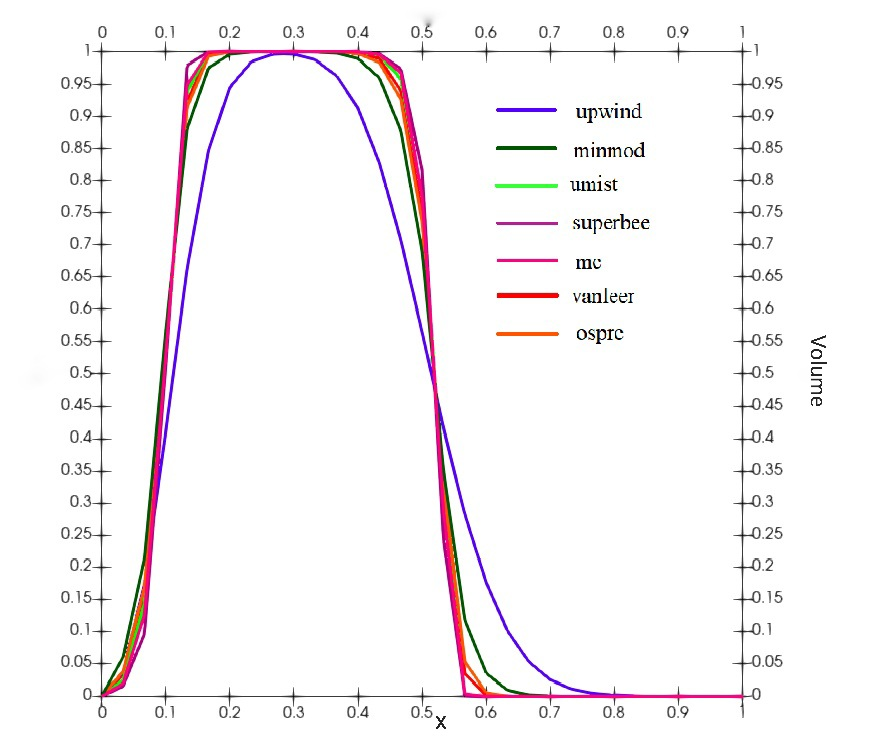
\includegraphics[width=0.6\linewidth]{03.jpeg}
    \caption{Распределение объёма в момент 0.3}
    \label{03}
\end{figure}

\begin{figure}[h!]
    \centering
     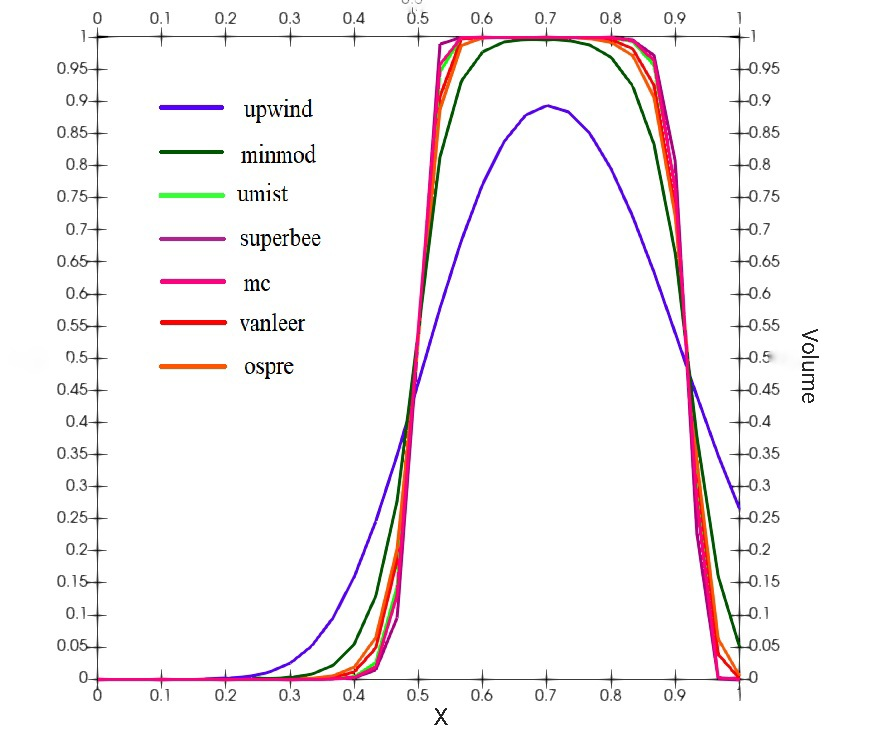
\includegraphics[width=0.6\linewidth]{07.jpeg}
    \caption{Распределение объёма в момент 0.7}
    \label{07}
\end{figure}


\begin{figure}[h!]
    \centering
     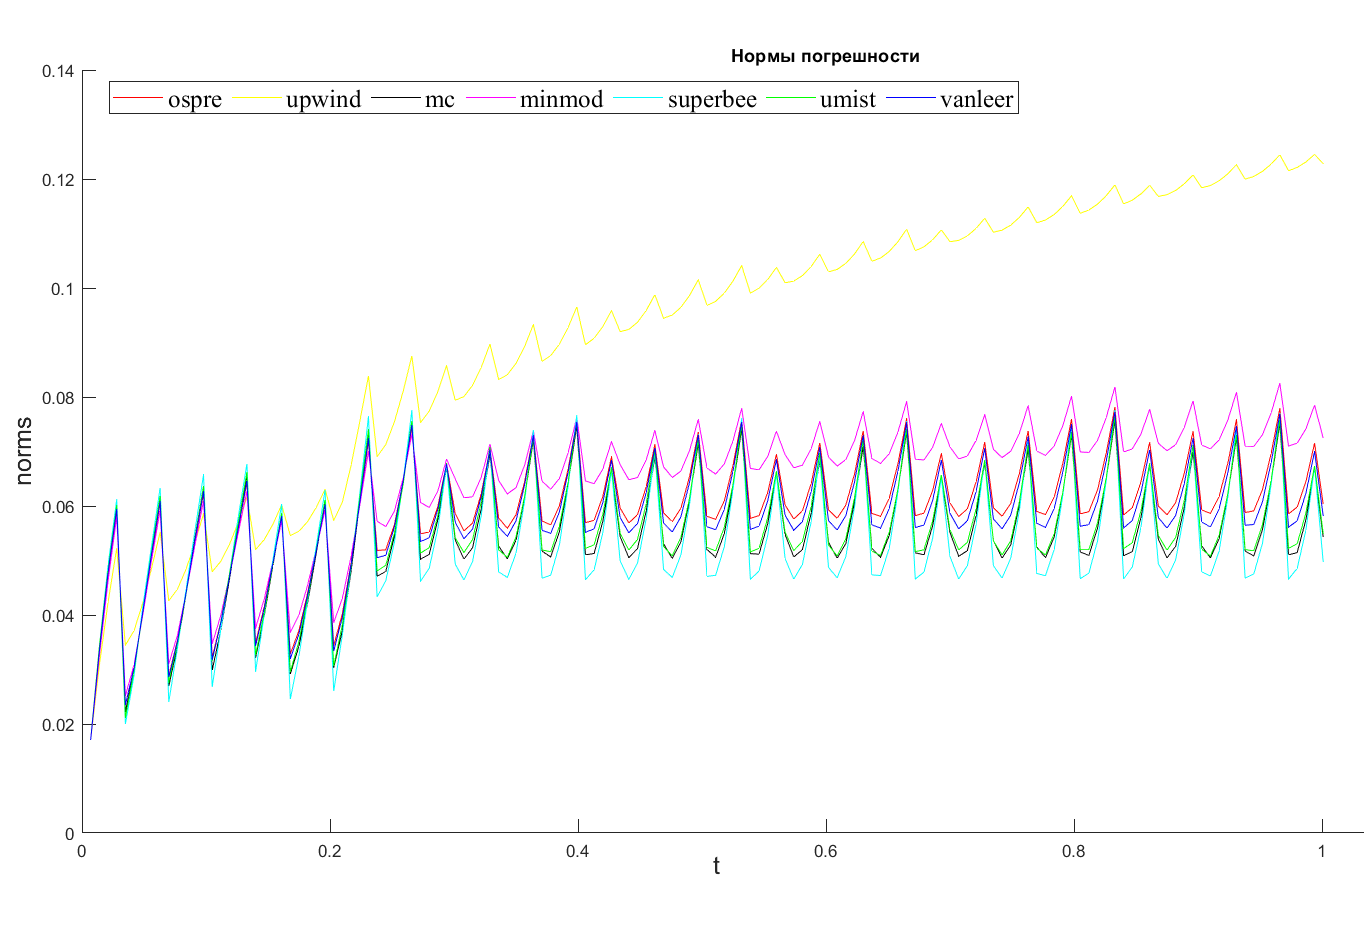
\includegraphics[width=1\linewidth]{norm.png}
    \caption{График погрешностей.}
    \label{norms}
\end{figure}

\begin{table}[h]
\centering
\caption {Значения погрешностей в момент 0.56 численного решения уравнения переноса}
\label{tab:norms_transport}
\begin{tabular}{|l|l|c|c|c|c|c|c|c|c|}
\hline
Ограничитель & Значение \\
\hline
SuperBee & 0.0659053\\
\hline
MC &  0.0659238\\
\hline
Umist & 0.0663728\\
\hline
Van Leer & 0.0685166\\
\hline
Ospre &  0.069493\\
\hline
MinMod & 0.0737164\\
\hline
Upwind  & 0.103783\\
\hline
\end{tabular}
\end{table}


На основе полученных данных можем сделать вывод, что для моделирования данной задачи не стоит использовать такие ограничители, как
Upwind и MinMod, а самыми точными оказались SuperBee и MC.
\clearpage
{\bf Тестовая задача: уравнение Бюргерса.} Рассмотрим уравнение вида
$$
\dfrac{\partial u(x, t)}{\partial t}+\dfrac12\dfrac{\partial u^2(x, t)}{\partial x} = 0
$$
с начальными условиями
$$
u(x, 0) = \begin{cases}
	1 - (x-1)^2, \quad \left|x-1\right| \leq 1,\\
	0, \quad \left|x-1\right| > 1.
\end{cases}
$$
Точное решением этой задачи на моменты времени $t<0.5$ будет иметь вид
$$
u_e = 1-\frac{{{\left( 1-\sqrt{1+4 t\, \left( t-x+1\right) }\right) }^{2}}}{4 {{t}^{2}}}
$$

Задача решалась с шагом по пространству  $h=0.1$ и шагом по времени $\tau=0.025$.
На рисунке \ref{fig:burgers} и в таблице \ref{tab:burgers} представлены решения и среднеквадратичные отклонения, полученные с использованием различных ограничителей.
Также как и в случае с задачей о бегущей волне, наиболее близкие к точному решению удалось получить с использованием ограничителя Superbee.

\begin{figure}[h]
\centering
\includegraphics[width=0.5\linewidth]{burgers.png}
\caption{Сравнение численного и точного решений уравнения Бюргерса на момент $t=0.5$}
\label{fig:burgers}
\end{figure}

\begin{table}[h]
\centering
\caption {Значения погрешностей в момент $t=0.5$ численного решения уравнения Бюргерса}
\label{tab:norms_burgers}
\begin{tabular}{|l|l|}
\hline
Ограничитель & Значение \\
\hline
SuperBee & 0.025357\\
\hline
Van Leer & 0.0279678\\
\hline
Upwind  & 0.050419\\
\hline
\end{tabular}
\end{table}

\clearpage
{\bf Тестовая задача: задача об одиночном импульсе.}
Рассмотрим задачу (\ref{sys_of_eq1}) о течении в канале с физическими параметрами, представленными в 
таблице \ref{tab:single_impulse_params}.

\begin{table}[h]
\centering
\caption {Параметры задачи об одиночном импульсе}
\label{tab:single_impulse_params}
\begin{tabular}{|l|l|}
\hline
$L$ & 2 м \\
\hline
$A_0$ & $\pi$ см$^2$\\
\hline
$h$ & $1.5$ мм\\
\hline
$\rho$  & 1050 кг/м$^3$\\
\hline
$\mu$  & 0 или 4 мПа$\cdot$с\\
\hline
$\zeta$  & 9\\
\hline
$E$  & 4$\cdot10^5$ Па\\
\hline
\end{tabular}
\end{table}

В качестве входного расхода используем функцию
$$
Q(t) = 10^{-6} \exp\left(-10^{-4}(t-0.05)^2\right) \quad m^3/s
$$
имеющую вид импульса с максимальным значением $10^{-6}$ м$^3$/с в момент времени $t=0.05$ сек.

В результате обезразмерирования получим следующие значения безразмерных комплексов, входящих в определяющую систему
$$
M_f = 0 \text{ или } 263.295,\quad  M_p = 7.5\cdot10^{6}.
$$

Задача решалась с шагом по пространству $h=5\cdot10^{-4}$ и шагом по времени $\tau=2 \cdot 10^{-5}$.
Численное решение на момент времени $t=10^{-3}$ представлено на рисунке \ref{fig:single_pulse_result}.

\begin{figure}[h]
\centering
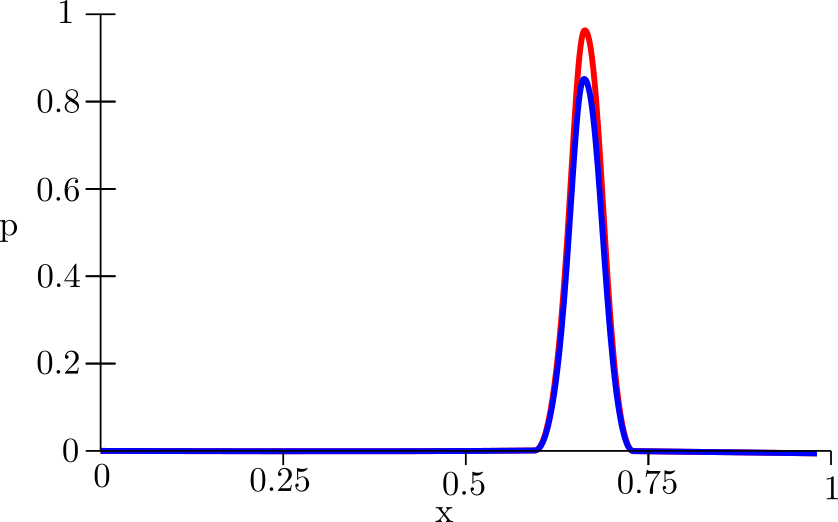
\includegraphics[width=0.5\linewidth]{single_pulse.png}
\caption{Значение давления для задачи одиночного импульса на момент $t=10^{-3}$. Красная линия соответствует параметру $M_f=0$, синяя -- $M_f=263.295$}
\label{fig:single_pulse_result}
\end{figure}


\newpage
\printbibliography

\end{document}
